\documentclass[paper,twocolumn]{geophysics}
%\documentclass[manuscript]{geophysics}
%\documentclass[manuscript,endfloat]{geophysics}
\usepackage{graphicx}
\newcommand{\mitbf}[1]{\mathbf{{#1}}}

\begin{document}

\title{Title}
\lefthead{Meh}
\righthead{Meh}
% manuscript number
\ms{Submission}

\renewcommand{\thefootnote}{\fnsymbol{footnote}}
\address{
\footnotemark[1] Universidade do Estado do Rio de Janeiro,
Rio de Janeiro, Brazil.
\\
\footnotemark[2] Observat\'orio Nacional,
Rio de Janeiro, Brazil.
\\
\footnotemark[3] Department of Mathematics and Geosciences,
University of Trieste, Trieste, Italy.
}

\author{
    Leonardo Uieda\footnotemark[1]\footnotemark[2]
    Val\'eria C. F. Barbosa\footnotemark[2],
    Vanderlei C. Oliveira Jr\footnotemark[2],
    and
    Carla Braitenberg\footnotemark[3]
}

\maketitle

\begin{abstract}
\end{abstract}

%%%%%%%%%%%%%%%%%%%%%%%%%%%%%%%%%%%%%%%%%%%%%%%%%%%%%%%%%%%%%%%%%%%%%%%%%%%%%%
\section{Introduction}


We use the optimized formula of \citet{Grombein2013} with Cartesian integral
kernels.

The Cartesian kernels are faster to compute.

The Cartesian kernels don't have singularities in the poles.

The traditional spherical integral kernels suffer from a singularity at the
poles \citep{Heck2007, Wild-Pfeiffer2008}.

The Cartesian formula are numerically integrated using a Taylor series
expansion as proposed by \citet{Heck2007}.

The Taylor series expansion approach produces accurate results at low
latitudes.

The Taylor series expansion presents a decrease in accuracy towards the polar
regions.

The tesseroids have an approximately rectangular surface area at low latitudes
but collapse into an approximately triangular shape at the poles.

\citet{Grombein2013} use a near-zone separation to mitigate the increased error
in high latitudes.

In the so called "near-zone" of the computation point they use a finner
discretization with smaller tesseroids.

This is accomplished by dividing the tesseroids along the horizontal
dimensions.

The determination of an optimal size of the near-zone remains an open question
\citep{Grombein2013}.

We use the Gauss-Legendre Quadrature (GLQ) to numerically integrate the Cartesian
kernels instead of the Taylor series expansion \citep{Asgharzadeh2007}.

The GLQ integration consists of approximating the volume integral by a weighted sum of
the effect of point masses.

The point masses are distributed according to the roots of Legendre polynomials
\citep{Hildebrand1987}.

An advantage of the GLQ approach is that the accuracy of integration can be
controlled by the number of point masses used.

A disadvantage of the GLQ is the increased computation time as the number of
point masses increases.

There is a trade-off between accuracy and computation time.

\citet{Ku1977} suggests that the accuracy of the GLQ integration depends on
the ratio between distance to the computation point and the distance between
adjacent point masses.

\citet{Ku1977} proposes an empirical criteria that the distance between adjacent
point masses should be less than the distance to the computation point.

This empirical criteria was used by \citet{Asgharzadeh2007} as a way to
choose the number of point masses used in the GLQ integration.

They suggested using this criteria for gravitational attraction as well as
the gravity gradient tensor (or Marussi tensor) of a tesseroid.

\citet{Ku1977} presented results for the vertical component of the
gravitational acceleration ($g_z$) caused by a right rectangular prism.

To our knowledge, there has been no investigation if the empirical criteria of
\citet{Ku1977} is valid for the second derivatives of the
gravitational potential.

There has also been no attempt to quantify the error committed in the GLQ
integration of gravity gradients when applying the criteria of \citet{Ku1977}.

\citet{Li2011} devised an automatic algorithm to enforce the criteria of
\citet{Ku1977}.

Their algorithm keeps the number of points masses per tesseroid fixed.

They then check the ratio between the minimum distance to the computation point
and the largest dimension of the tesseroid.

If the ratio below a specified threshold value, the tesseroid is divided into
smaller tesseroids.

This division is repeated recursively until all tesseroids obey the criteria.

The GLQ integration is then performed for each of the smaller tesseroids
using the fixed number of point masses.

The algorithm of \citet{Li2011} is similar to the near-zone separation used by
\citet{Grombein2013}.

The advantage of the adaptive discretization of \citet{Li2011} over simply
increasing the number of points masses in the GLQ is that the
amount of point masses will be greater only close to the computation point.

This makes the adaptive discretization more computationally efficient.


We will attempt to quantify the error committed in the computation of the
gravity gradients using the GLQ with adaptive discretization.

We will establish an empirical relationship between the integration error and
the ratio between the distance to the computation point and the dimensions of
the tesseroid.

This will allow one to choose the appropriate amount of discretization to
achieve the desired accuracy.


%%%%%%%%%%%%%%%%%%%%%%%%%%%%%%%%%%%%%%%%%%%%%%%%%%%%%%%%%%%%%%%%%%%%%%%%%%%%%%
\section{Theory}

\citet{Grombein2013} provides Cartesian kernels for the tesseroid volume
internals that define the gravitational potential, gravitational attraction,
and Marussi tensor (EQUATIONS).
\begin{equation}
    V(r,\phi,\lambda) = G \rho
        \int\limits_{\lambda_1}^{\lambda_2}
        \int\limits_{\phi_1}^{\phi_2}
        \int\limits_{r_1}^{r_2}
        \frac{1}{\ell} \kappa  dr' d\phi' d\lambda',
    \label{eq:tesspot}
\end{equation}
\begin{equation}
    g_{\alpha}(r,\phi,\lambda) = G \rho
        \int\limits_{\lambda_1}^{\lambda_2}
        \int\limits_{\phi_1}^{\phi_2}
        \int\limits_{r_1}^{r_2}
        \frac{\Delta\alpha}{\ell^3} \kappa dr' d\phi' d\lambda',
    \label{eq:tessgrav}
\end{equation}
\noindent
and
\begin{equation}
    g_{\alpha\beta}(r,\phi,\lambda) = G \rho
        \int\limits_{\lambda_1}^{\lambda_2}
        \int\limits_{\phi_1}^{\phi_2}
        \int\limits_{r_1}^{r_2}
        I_{\alpha\beta}
        dr' d\phi' d\lambda',
    \label{eq:tesstensor}
\end{equation}

We will follow \citet{Asgharzadeh2007} and perform the numerical integration
using the Gauss-Legendre Quadrature (GLQ).

The GLQ consists of approximating the integral by a weighted sum of the
integration kernel \citep{Hildebrand1987},
\begin{equation}
    \int\limits_a^b f(x) dx \approx
    \frac{b-a}{2}\sum\limits_{i=1}^N W_i f(x_i),
    \label{eq:glq1d}
\end{equation}

$N$ is the order of the quadrature, i.e. the number of points used in the GLQ.

The points $x_i$ where the kernel is evaluated are called the quadrature nodes.

The points are roots of the $N^{th}$ order Legendre polynomial $P_N(x)$.

The roots are $x = \pm 0.577350269$ for a second order polynomial ($P_2(x)$).

A root finder algorithm can be used to determine the roots for larger order
polynomials.

We refer the reader to \citet{Barrera-Figueroa2006} for an algorithm tailored
for Legendre polynomials in particular.

The second order roots, as well as the ones determined by a root finder
algorithm, will be within the range $[-1, 1]$.

Thus, the roots must be scaled to the integration limits $[a, b]$ by
\begin{equation}
    x^{scaled}_i = \frac{b - a}{2} x_i + \frac{b + a}{2}.
\end{equation}

The weights of the GLQ are given by \citep{Hildebrand1987},
\begin{equation}
    W_i = \frac{2}{(1 - x_i^2)(P^\prime_N(x_i))^2},
\end{equation}

The values of the $P_N(x)$ and its first derivative $P^\prime_N(x)$ can be
calculated with recursive relations (PUT FORMULA HERE?).

The Gauss-Legendre Quadrature for volume integrals, like equations
\ref{eq:tesspot}, \ref{eq:tessgrav}, and \ref{eq:tesstensor},
becomes \citep{Asgharzadeh2007} (EQUATION).

Applying equation (GLQ 3D) to equations
\ref{eq:tesspot}, \ref{eq:tessgrav}, and \ref{eq:tesstensor},
we see that $f(r_i, \phi_j, \lambda_k)$ is the effect of a point
mass located on the quadrature nodes.

It can be said that the GLQ integration approximates the volume integrals  by a
weighted sum of point mass effects.


The accuracy of the integration
depends on the number of point masses used in the summation.

\citet{Ku1977} showed that it also depends on the ratio between
the distance to the computation point and the distance between adjacent nodes.

Figure~\ref{fig:glqerrorsample}
illustrates this effect on the $g_{xy}$ gravity gradient component.

The $g_{xy}$ component was produced by a
$7^\circ \times 7^\circ \times 20\ km$ tesseroid
with $2.67\ g.cm^{-3}$ density
and top at $z=0\ km$.

The maps were calculated on a regular grid
with $100\times100$ points.

The GLQ order used was the same
in the radial, longitudinal, and latitudinal dimensions.

Figure~\ref{fig:glqerrorsample}a shows the $g_{xy}$ component
calculated at 400 km height using
GLQ with order two (two point masses in the longitude, latitude, and vertical
directions, respectively).

Figure~\ref{fig:glqerrorsample}b shows $g_{xy}$ computed with order two
GLQ as well but at 150 km height.

Notice that the computed effect is concentrated around each point mass (black
dots) and does not resemble the effect of a tesseroid.

\citet{Ku1977} determined an empirical criterion that the distance between
point masses (quadrature nodes) should be smaller than the minimum distance to
the computation point.

Thus, if a computation point is too close to the tesseroid one would have to
decrease the distance between the point masses in order to obtain an accurate
result.

One way to accomplish this would be increase the order of the quadrature
$N$ in all three directions.

Figure~\ref{fig:glqerrorsample}c shows the $g_{xy}$ component calculated at
150km height but with a GLQ order of 30.

\begin{figure}
    \centering
    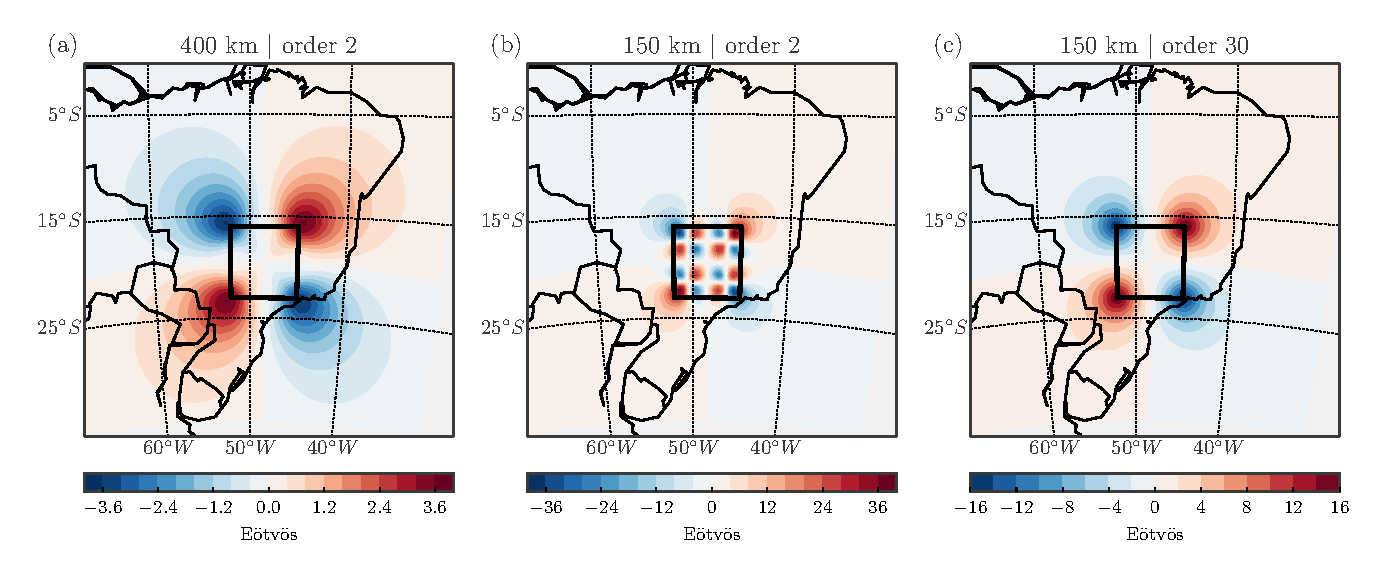
\includegraphics[width=\textwidth]{figs/vary-height-and-order}
    \caption{
        Example of the effect of varying
        the computation height
        and the number of point masses in the Gauss-Legendre Quadrature
        (i.e., the GLQ order).
        Black circles represent the horizontal location of the GLQ nodes
        (not shown for GLQ order 30).
        a) Field calculated at $400\ km$ height using GLQ order 2.
        The effect is similar to that presented by \citet{Asgharzadeh2007}.
        b) At $150\ km$ height and order 2,
        the field resembles that of
        four point sources located at the GLQ nodes.
        This effect was shown by \citet{Ku1977}
        for the case of the $g_z$ component of a right rectangular prism.
        c) At $150\ km$ but with a higher GLQ order of 30,
        the field is similar to that expected for a single mass source.
    }
    \label{fig:glqerrorsample}
\end{figure}





\subsection{Adaptive discretization}


\citet{Li2011} proposed an alternative way to decrease the distance between
point masses and achieve an accurate integration.

Instead of increasing the GLQ order,
they divide the tesseroid into smaller tesseroids while keeping the number of
point masses per tesseroid fixed.

The gravitational effect of the larger tesseroid would be calculated as the sum
of the effects of the eight smaller tesseroids.

This division would effectively decrease the distance between nodes because of
the smaller tesseroids.

The criterion for dividing a tesseroid is that
the distance to the computation point must be smaller than
a constant times the size of the tesseroid.

The size of the tesseroid is used as proxy for the distance between point
masses.

This procedure is repeated recursively
(i.e., to each of the smaller tesseroids)
until all tesseroids are within the acceptable distance-size ratio
or a minimum size is achieved.


The advantage of this adaptive discretization is that the number of point
masses is only increased in regions of the tesseroid that are closer to the
computation point.

Alternatively, simply increasing the order of the GLQ would increase the number
of point masses evenly throughout the whole tesseroid.


%%%%%%%%%%%%%%%%%%%%%%%%%%%%%%%%%%%%%%%%%%%%%%%%%%%%%%%%%%%%%%%%%%%%%%%%%%%%%%
\section{Implementation}


%%%%%%%%%%%%%%%%%%%%%%%%%%%%%%%%%%%%%%%%%%%%%%%%%%%%%%%%%%%%%%%%%%%%%%%%%%%%%%
\section{Numerical evaluation of the accuracy}

The key controlling point of their algorithm is the ratio between
the smallest distance to the computation point and
the largest side length of the tesseroid.

The value of this ratio is used to decide whether a tesseroid will be divided
or not.

Thus, the value chosen for the minimum allowed value of this ratio determines
how many divisions are made.

Consequently, the value for the minimum distance-size ratio controls both the
accuracy of the integration and the computation time.

\citet{Li2011} provide a few examples of values for this ratio in the case of
the vertical component of gravitational attraction.

However, there has been no further investigation into
the relationship between values of the minimum distance-size
ratio and the computation error.

It is also not clear whether the same relationship holds for the gravitational
attraction as well as for the gradient tensor components.


%%%%%%%%%%%%%%%%%%%%%%%%%%%%%%%%%%%%%%%%%%%%%%%%%%%%%%%%%%%%%%%%%%%%%%%%%%%%%%
\section{Results}


%%%%%%%%%%%%%%%%%%%%%%%%%%%%%%%%%%%%%%%%%%%%%%%%%%%%%%%%%%%%%%%%%%%%%%%%%%%%%%
\section{Discussion}

%%%%%%%%%%%%%%%%%%%%%%%%%%%%%%%%%%%%%%%%%%%%%%%%%%%%%%%%%%%%%%%%%%%%%%%%%%%%%%
\section{Conclusions}

%%%%%%%%%%%%%%%%%%%%%%%%%%%%%%%%%%%%%%%%%%%%%%%%%%%%%%%%%%%%%%%%%%%%%%%%%%%%%%
\section{Acknowledgments}


\bibliographystyle{seg}
\bibliography{references.bib}
\end{document}
